\chapter{Результаты проектирования архитектуры модуля для оркестрации
Kubernetes}


\section{Описание архитектуры модуля для развертывания Terraform}

В данном разделе представлено описание архитектуры модулей, которые включают в
себя "Case Classes Generator", "HCL Generator", "HCL Deployer", "Autoscaler" и
"Config Parser". Эти модули взаимодействуют друг с другом для обеспечения
функциональности приложения.

\subsection{Case Classes Generator}

Первый модуль, "Case Classes Generator" (см. Рисунок \ref{fig:ccg}), отвечает за
получение метаданных и формирование case classes. Этот модуль принимает на вход
данные от "Plugin Analyzer" и "Docs Analyzer", которые анализируют плагины и
документацию соответственно. Результатом работы этого модуля являются
сгенерированные case classes, которые затем передаются в "HCL Generator".

\begin{figure}[h]
  \centering
  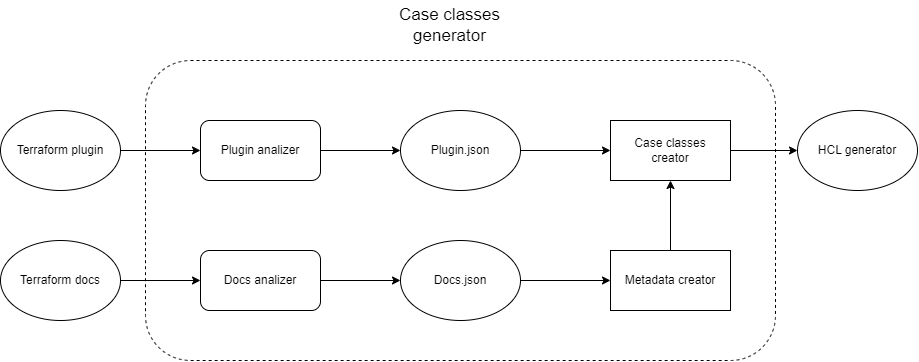
\includegraphics[scale=0.5]{img/1.png}
  \caption{Архитектура модуля "Case Classes Generator"}
  \label{fig:ccg}
\end{figure}

\subsection{HCL Generator}

"HCL Generator" (см. Рисунок \ref{fig:hclg}) является вторым модулем и не имеет
собственной точки входа. Он получает case classes от "Case Classes Generator" и
генерирует из них HCL конфигурацию. Этот модуль является ключевым для получения
HCL конфига и его последующего запуска.

\begin{figure}[h]
  \centering
  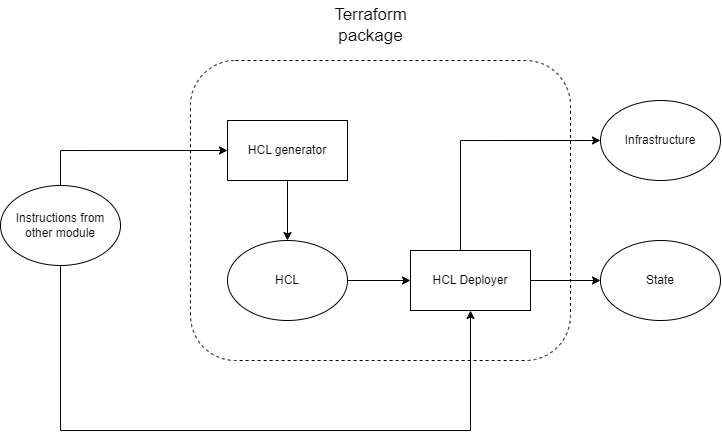
\includegraphics[scale=0.6]{img/2.png}
  \caption{Архитектура модуля "HCL Generator"}
  \label{fig:hclg}
\end{figure}

\subsection{HCL Deployer и Autoscaler}

Третий модуль, "HCL Deployer" (см. Рисунок \ref{fig:hdas}), использует HCL
конфигурацию, сгенерированную "HCL Generator", для изменения архитектуры
кластера. Он также подключается к API Kubernetes для получения состояния
кластера и принятия решений о масштабировании, а также перемещения pods с одной
node на другую. Этот модуль завернут в Helm chart и его следует запускать на
master node кластера для автоматического масштабирования кластера.

\begin{figure}[h]
  \centering
  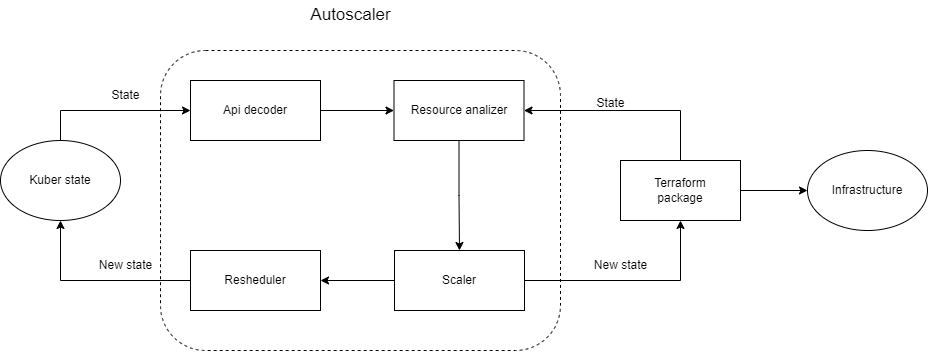
\includegraphics[scale=0.5]{img/3.png}
  \caption{Архитектура модулей "HCL Deployer" и "Autoscaler"}
  \label{fig:hdas}
\end{figure}

\vspace{15mm}

\subsection{Config Parser}

Четвертый модуль, "Config Parser" (см. Рисунок \ref{fig:cp}), использует HCL
конфигурацию для развертывания кластера с запущенным на нем модулем "HCL
Deployer", а также для первичной настройки модуля "HCL Deployer" и архитектуры
кластера. 

\begin{figure}[h]
  \centering
  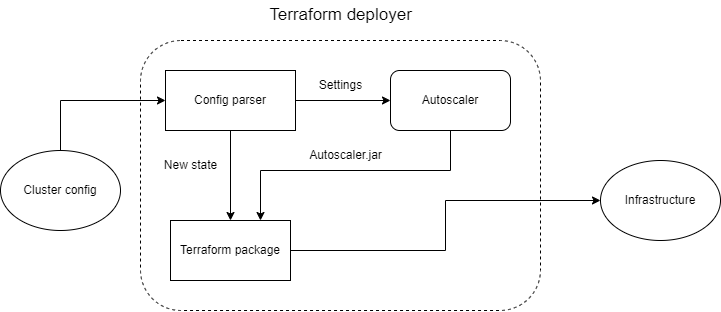
\includegraphics[scale=0.6]{img/4.png}
  \caption{Архитектура модуля "Config Parser"}
  \label{fig:cp}
\end{figure}

\section{Разработка интерфейсов и классов модуля для генерации HCL конфигурации}

В процессе разработки модуля-обертки для развертывания типизированных
определений Terraform, было необходимо создать ряд интерфейсов и классов,
которые обеспечивают структуру и функциональность модуля. Эти интерфейсы и
классы были разработаны с учетом особенностей работы Terraform и требований к
типизации и структуре данных.

В основе архитектуры модуля лежат следующие интерфейсы и классы:

\begin{itemize}
\item $ProviderType$: Этот интерфейс представляет тип провайдера в
Terraform. Он служит базовым интерфейсом для всех конкретных типов провайдеров.

\item $TerraformResource$: Этот абстрактный класс представляет ресурс в
Terraform. Он содержит метод $toHCL$, который должен быть реализован в
каждом конкретном классе ресурса для преобразования объекта ресурса в его HCL
представление.

\item $InfrastructureResource[T <: ProviderType]$: Этот интерфейс
расширяет \newline $TerraformResource$ и представляет ресурс инфраструктуры в
Terraform. Он параметризован типом провайдера.

\item $ProviderSettings[T <: ProviderType]$: Этот интерфейс расширяет
\newline $TerraformResource$ и представляет настройки провайдера в Terraform.
Он также параметризован типом провайдера.

\item $BackendResource$: Этот интерфейс расширяет
$TerraformResource$ и представляет ресурс бэкенда в Terraform.

\item $ProviderConfig[A, T_1, T_2, T_3]$: 
$A <: ProviderType, T_1 <: ProviderSettings[A], T_2 <:
BackendResource, T_3 <: InfrastructureResource[A]$. 
Этот класс представляет конфигурацию провайдера в Terraform.
Он содержит все необходимые данные для создания и развертывания
конфигурации провайдера, включая настройки провайдера,
ресурс бэкенда и ресурсы инфраструктуры. Он также содержит метод $toHCL$
для преобразования конфигурации провайдера в его HCL представление.
\end{itemize}

Для успешного проектирования модуля было необходимо разработать механизмы для
извлечения информации о структуре определений ресурсов и источников данных из
Terraform. Это было достигнуто путем создания специальных компонентов, которые
выполняют следующие функции:

\begin{itemize}
  \item Получение структуры ресурсов из определения плагина Terraform:
Этот компонент отвечает за анализ определений плагина Terraform, написанных на
языке Go, и извлечение из них структуры ресурсов. Это включает в себя информацию
о типах ресурсов, их свойствах и связях между ними.
  
  \item Анализ документации и получение из нее полезной информации:
Этот компонент отвечает за анализ документации Terraform и извлечение из нее
полезной информации. Это может включать в себя дополнительные свойства полей,
которые не могут быть получены из анализа определений плагина, такие как
возможность содержания полем типа JSON или ID.
  
  \item Преобразование полученных данных в формат JSON: После
извлечения информации о структуре ресурсов и анализа документации, эта
информация преобразуется в формат JSON для дальнейшего использования. Это
включает в себя создание двух файлов JSON, каждый из которых содержит информацию
о структуре ресурсов и источников данных.
  
  \item Передача полученных данных в основной модуль на Scala: После
преобразования данных в формат JSON, они передаются в основной модуль на Scala.
Этот модуль затем использует эти данные для создания case classes, с
определенной на них функцией toHCL, которые представляют собой типизированные
определения Terraform.
\end{itemize}

\section{Разработка функций для взаимодействия с Kubernetes}

\subsection{Общее описание функций и типов модуля}

Для взаимодействия с Kubernetes необходимо разработать следующие типы, которые
будут хранить конфигурацию всего кластера:

\begin{itemize}
\item \textbf{Node}: Этот тип представляет собой узел в кластере Kubernetes.
Узел может быть виртуальной или физической машиной в зависимости от кластера.
\item \textbf{Pod}: Pod в Kubernetes - это наименьшая и простейшая единица в
модели объектов Kubernetes, которую создает или развертывает пользователь. Pod
представляет собой группу одного или нескольких контейнеров, которые разделяют
хранилище и сетевые ресурсы, и спецификация о том, как запускать контейнеры.
\item \textbf{Event}: События в Kubernetes представляют собой объекты, которые
предоставляют представление о том, что происходит внутри кластера, например,
какие поды/узлы были запущены/остановлены и т.д.
\item \textbf{KuberInfo}: Этот тип представляет собой общую информацию о
кластере Kubernetes, такую как количество узлов, подов, событий и т.д.
\end{itemize}

Также необходимо разработать следующие функции:

\begin{itemize}
\item \textbf{drainNodes}: Функция для удаления подов с узлов.
\item \textbf{processResources}: Функция для обработки ресурсов в Kubernetes.
\item \textbf{increaseReplicas}: Функция для увеличения количества реплик в
ресурсе.
\item \textbf{cordonNode}: Функция для установки узла в режим "не планируемый",
что означает, что на него не будут назначены новые поды.
\item \textbf{getResources}: Функция для получения списка всех ресурсов в
кластере.
\item \textbf{getAutoscaler}: Функция для получения информации об
автомасштабировании для определенного развертывания.
\item \textbf{disableAutoscaler}: Функция для отключения автомасштабирования для
определенного развертывания.
\item \textbf{enableAutoscaler}: Функция для включения автомасштабирования для
определенного развертывания.
\item \textbf{deletePod}: Функция для удаления пода.
\item \textbf{waitUntilAllPodsVerified}: Функция для ожидания, пока все поды не
будут проверены и не начнут работать.
\end{itemize}

Пожалуйста, обратите внимание, что все эти функции предполагают наличие
экземпляра KubernetesClient, который предоставляет методы для взаимодействия с
API Kubernetes. Эти функции используются для управления ресурсами в кластере
Kubernetes, включая узлы, поды, репликации и автомасштабирование.

Все функции возвращают результат в виде IO, что позволяет обрабатывать
асинхронные операции и ошибки в функциональном стиле.

Важно отметить, что эти функции представляют собой общий интерфейс для
взаимодействия с Kubernetes и могут быть расширены или модифицированы в
соответствии с конкретными требованиями приложения.

\subsection{Работа Scaler}

Scaler является ключевым компонентом в системе, который отвечает за
автоматическое масштабирование ресурсов в Kubernetes. Он использует информацию
из KuberInfo для определения текущего состояния кластера и принятия решений о
масштабировании.

\begin{itemize}
\item \textbf{Проверка возможности перемещения подов}: Scaler анализирует
текущее распределение подов по узлам и определяет, можно ли переместить поды
таким образом, чтобы один или несколько узлов были полностью освобождены. Это
может быть полезно для оптимизации использования ресурсов или подготовки узла к
обслуживанию или удалению. При этом Scaler учитывает ресурсы, необходимые для
поддержания работоспособности каждого пода, чтобы гарантировать, что после
перемещения все поды смогут корректно функционировать.

\item \textbf{Проверка наличия достаточных ресурсов}: Scaler также проверяет,
нет ли ситуации, когда под не может быть запущен из-за нехватки ресурсов. Это
может произойти, если все узлы в кластере загружены или если под требует больше
ресурсов, чем доступно на любом из узлов. В таком случае Scaler может принять
решение о масштабировании узлов, чтобы обеспечить достаточность ресурсов для
всех подов.
\end{itemize}

Важно отметить, что действия Scaler зависят от конкретной политики
масштабирования, которая может варьироваться в зависимости от требований
приложения и конфигурации кластера. Например, некоторые системы могут
предпочитать минимизировать количество используемых узлов для снижения затрат, в
то время как другие могут стремиться максимизировать распределение нагрузки для
повышения отказоустойчивости.

\section{Разработка функций для взаимодействия с Terraform и Kubernetes}

Для эффективного взаимодействия между Terraform и Kubernetes необходимо
установить соответствие между серверами, объявленными в Terraform, и узлами
(Nodes) в Kubernetes. Это соответствие, или биекция, позволяет нам управлять и
изменять конфигурацию обоих систем согласованно.

\subsection{Установление биекции}

Биекция между серверами Terraform и узлами Kubernetes позволяет нам точно знать,
какой сервер Terraform соответствует какому узлу Kubernetes. Это важно,
поскольку обе системы имеют разные представления об инфраструктуре и управляют
ею по-разному. Установление такого соответствия позволяет нам синхронизировать
состояние обоих систем.

Для установления этого соответствия мы вводим специальные теги при создании
серверов в конфигурации Terraform. Эти теги позволяют нам однозначно
идентифицировать каждый сервер и узел, обеспечивая точное соответствие между
ними.

Важно отметить, что все эти операции должны быть автоматизированы и
синхронизированы, чтобы обеспечить согласованность и надежность нашей
инфраструктуры. Это может потребовать разработки дополнительных функций или
скриптов, которые будут отслеживать состояние обоих систем и автоматически
применять необходимые изменения при обнаружении отклонений от желаемого
состояния.

\section{Выводы}

В ходе проектирования архитектуры модуля-обертки для развертывания
типизированных определений Terraform были разработаны и описаны ключевые
компоненты системы, включая "Case Classes Generator", "HCL Generator", "HCL
Deployer", "Autoscaler" и "Config Parser". Эти модули взаимодействуют друг с
другом для обеспечения функциональности приложения, включая генерацию HCL
конфигурации, развертывание и масштабирование инфраструктуры, а также анализ и
обработку конфигурации.

Были разработаны интерфейсы и классы для генерации HCL конфигурации, включая
ProviderType, TerraformResource, InfrastructureResource, ProviderSettings,
BackendResource и ProviderConfig. Эти интерфейсы и классы обеспечивают гибкость
и расширяемость системы, позволяя поддерживать различные типы провайдеров и
ресурсов.

Для взаимодействия с Kubernetes были разработаны типы Node, Pod, Event и
KuberInfo, а также функции для управления узлами и подами, масштабирования
ресурсов и анализа состояния кластера. Эти функции предоставляют общий интерфейс
для взаимодействия с Kubernetes и могут быть расширены или модифицированы в
соответствии с конкретными требованиями приложения.

Была реализована биекция между серверами Terraform и узлами Kubernetes,
позволяющая синхронизировать состояние обоих систем и управлять их конфигурацией
согласованно. Для установления этого соответствия были введены специальные теги
при создании серверов в конфигурации Terraform.

В целом, разработанная архитектура модуля-обертки для развертывания
типизированных определений Terraform обеспечивает эффективное взаимодействие
между Terraform и Kubernetes, позволяя автоматизировать процесс развертывания и
управления инфраструктурой.